% \begin{tikzpicture}
\node at (0,0) {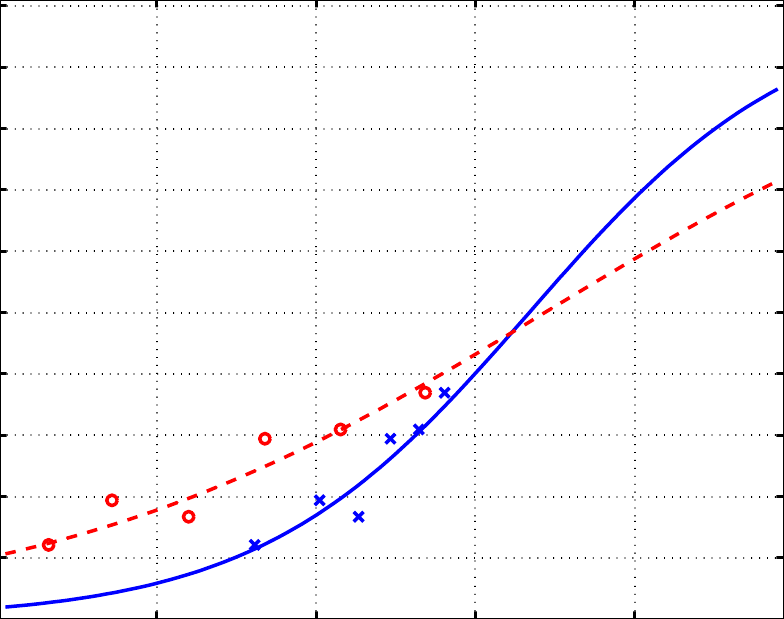
\includegraphics[width=6cm]{img/chap4/farias2}};
% \draw (-3,-2.36) rectangle (3,2.35);

\def\shiftX{-2.5}
\def\shiftY{2}

\draw[legende] (-0.2+\shiftX,-0.1+\shiftY) rectangle (2.9+\shiftX,-2.2+\shiftY);
\draw (2.6+\shiftX,-0.4+\shiftY) node[anchor=east,font=\scriptsize] {modèle synthétique};
\draw (2.6+\shiftX,-0.9+\shiftY) node[anchor=east,font=\scriptsize] {données synthétiques};
\draw (2.6+\shiftX,-1.4+\shiftY) node[anchor=east,font=\scriptsize] {modèle MPEG};
\draw (2.6+\shiftX,-1.9+\shiftY) node[anchor=east,font=\scriptsize] {données MPEG};
\fill[blue] (2.6+\shiftX,-0.45+\shiftY) rectangle (2.8+\shiftX,-0.4+\shiftY);
\fill[blue,rotate=135] (0.675,-0.825) rectangle (0.625,-1.025);
\fill[blue,rotate=135] (0.75,-0.9) rectangle (0.55,-0.95);
% \fill[blue,rotate=135] (-2.525,-1.175) rectangle (-2.575,-1.375);
% \fill[blue,rotate=135] (-2.45,-1.25) rectangle (-2.65,-1.3);
\fill[red] (2.6+\shiftX,-1.45+\shiftY) rectangle (2.8+\shiftX,-1.4+\shiftY);
\draw[thick,red] (2.7+\shiftX,-1.92+\shiftY) circle (0.07);

\node[anchor=north] at (-1.8,-2.3) {3};
\node[anchor=north] at (-0.55,-2.3) {3,5};
\node[anchor=north] at (0.65,-2.3) {4};
\node[anchor=north] at (1.85,-2.3) {4,5};
\node[below=0.3cm] at (0,-2.4) {$\mathit{LTSE}$};

\node[anchor=east] at (-2.9,-2.35) {0};
\node[anchor=east] at (-2.9,-1.9) {10};
\node[anchor=east] at (-2.9,-1.45) {20};
\node[anchor=east] at (-2.9,-1.05) {30};
\node[anchor=east] at (-2.9,-0.55) {40};
\node[anchor=east] at (-2.9,-0.1) {50};
\node[anchor=east] at (-2.9,0.45) {60};
\node[anchor=east] at (-2.9,0.85) {70};
\node[anchor=east] at (-2.9,1.4) {80};
\node[anchor=east] at (-2.9,1.85) {90};
\node[anchor=east] at (-2.9,2.3) {100};
\node[rotate=90] at (-3.8,0) {gêne moyenne};


% \end{tikzpicture}
